\subsection{COMPACTNESS OF UNIFORM SPACES}

DEFINITION 2. A uniform space X is said to be precompact if its Hausdorff completion \(\hat{\mathbf{X}}\) is compact. A subset A of a uniform space X is said to be a precompact subset if the uniform subspace A of X is precompact.

Thus a subset A of a uniform space X is precompact if and only if the closure of \(i(\mathbf{A})\) in \(\hat{X}\) is compact ( \(i: X \rightarrow \hat{X}\) being the canonical map) ( \(\S\) 3, no. 9, Proposition 18, Corollary 1).

Example. In any uniform space X, the set of points of a Cauchy sequence \((x_{n})\) is precompact. Since the images of the \(x_{n}\) in \(\hat{X}\) again form a Cauchy sequence, we can assume that X is Hausdorff; the closure in \(\hat{X}\) of the set of points \(x_{n}\) then consists of the points \(x_{n}\) and \(\lim_{n\to\infty}x_{n}\) and is therefore compact (Chapter I, § 9, no. 3, Example 2).

THEOREM 3. A uniform space X is precompact if and only if, for each entourage V of X, there is a finite covering of X by V-small sets.

We may express this condition more intuitively by saying that X can be covered by a finite number of sets which are as small as we please.

Let \(i: \mathbf{X} \to \hat{\mathbf{X}}\) be the canonical mapping, then the entourages of \(\mathbf{X}\) are the inverse images under \(i \times i\) of the entourages of \(\hat{\mathbf{X}}\) (§ 3, no. 7, Proposition 12). Suppose \(\mathbf{X}\) is precompact, and let \(\mathbf{U}\) be any entourage of \(\hat{\mathbf{X}}\) ; then there is a symmetric entourage \(\mathbf{U}'\) of \(\hat{\mathbf{X}}\) such that \(\hat{\mathbf{U}}' \subset \mathbf{U}\) . Since \(\hat{\mathbf{X}}\) is compact, there exist a finite number of points \(x_j \in \hat{\mathbf{X}}\) such that the \(\mathbf{U}'(x_j)\) (which are U-small) cover \(\hat{\mathbf{X}}\) . If \(\mathbf{V}\) is the inverse image of \(\mathbf{U}\) by \(i \times i\) , the sets \(i^{-1}(\mathbf{U}'(x_j))\) are V-small and cover \(\mathbf{X}\) . Conversely, suppose that for each entourage \(\mathbf{V}\) of \(\mathbf{X}\) there is a finite covering of \(\mathbf{X}\) by V-small sets. We have to show that every ultrafilter \(\mathfrak{F}\) on \(\hat{\mathbf{X}}\) is convergent; since \(\hat{\mathbf{X}}\) is complete, it is enough to show that \(\mathfrak{F}\) is a Cauchy filter, i.e.~that for each closed entourage \(\mathbf{U}\) of \(\hat{\mathbf{X}}\) there is a U-small set in \(\mathfrak{F}\) (§ 1, no. 2, Proposition 2, Corollary 2). Let \(\mathbf{V}\) be the inverse image of \(\mathbf{U}\) under \(i \times i\) , and let \((\mathbf{B}_j)\) be a finite covering of \(\mathbf{X}\) by V-small sets; then the sets \(C_j = i(B_j)\) are U-small and cover \(i(\mathbf{X})\) , so that

\[
\hat {\mathbf {X}} = \bigcup_ {j} \overline {{\mathbf {C}}} _ {j}.
\]

On the other hand, since \(\mathbf{C}_j \times \mathbf{C}_j \subset \mathbf{U}\) , and \(\mathbf{U}\) is closed in \(\hat{\mathbf{X}} \times \hat{\mathbf{X}}\) , we have \(\overline{\mathbf{C}}_j \times \overline{\mathbf{C}}_j \subset \mathbf{U}\) , so that the \(\overline{\mathbf{C}}_j\) are also \(\mathbf{U}\) -small. Since \(\mathfrak{F}\) is an ultrafilter, one of the \(\overline{\mathbf{C}}_j\) belongs to \(\mathfrak{F}\) (Chapter I, § 6, no. 4, Corollary to Proposition 5).

Q.E.D.

COROLLARY. A uniform space X is compact if and only if it is Hausdorff and complete and can be covered by a finite number of V-small sets, where V is any entourage of X.

This follows from Theorem 3 and Theorem 1 of no. 1.

Remark 1. A non-Hausdorff quasi-compact space is not necessarily uniformizable, since it need not satisfy axiom (O \(_{III}\) ) (cf.~Chapter I, § 9, no. 2); for example most of the non-Hausdorff quasi-compact spaces which appear in algebraic geometry do not satisfy axiom (O \(_{III}\) ) (cf.~Exercise 2).

PROPOSITION 1. In a uniform space every subset of a precompact set, every finite union of precompact sets and the closure of every precompact set are precompact.

The first two assertions are immediate consequences of Theorem 3. Let X be a uniform space, A a precompact subset of X, and let \(i: \mathbf{X} \to \hat{\mathbf{X}}\) be the canonical mapping. \(i(\overline{\mathbf{A}})\) is contained in the closure of \(i(\mathbf{A})\) in \(\hat{\mathbf{X}}\) (Chapter I, § 2, no. 1, Theorem 1), hence the closure of \(i(\overline{\mathbf{A}})\) in \(\hat{\mathbf{X}}\) is contained in a compact set and is therefore compact.

\pandocbounded{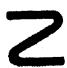
\includegraphics[keepaspectratio]{images/part002_3e3611b3.jpg}}

Remark 2. In a uniform space X a relatively compact set A is precompact, since A is contained in a compact set. On the other hand, even if X is Hausdorff, a precompact set need not be relatively compact in X, as is shown by the case where X itself is precompact but not compact.

PROPOSITION 2. Let \(f: \mathbf{X} \to \mathbf{Y}\) be a uniformly continuous mapping. If \(\mathbf{A}\) is any precompact subset of \(\mathbf{X}\) , then \(f(\mathbf{A})\) is a precompact subset of \(\mathbf{Y}\) . For if \(i: \mathbf{X} \to \hat{\mathbf{X}}\) and \(j: \mathbf{Y} \to \hat{\mathbf{Y}}\) are the canonical mappings, we have \(j(f(\mathbf{A})) = \hat{f}(i(\mathbf{A}))\) (§ 3, no. 7, Proposition 15) and hence \(j(f(\mathbf{A}))\) is relatively compact in \(\hat{\mathbf{Y}}\) (Chapter I, § 9, no. 4, Theorem 2, Corollary 1).

PROPOSITION 3. Let X be a set, let \((\mathrm{Y}_{\lambda})_{\lambda \in \mathbf{L}}\) be a family of uniform spaces, and for each \(\lambda \in L\) let \(f_{\lambda}\) be a mapping of X into \(Y_{\lambda}\) . Let X carry the coarsest uniformity for which the \(f_{\lambda}\) are uniformly continuous. Then a subset A of X is precompact if and only if \(f_{\lambda}(A)\) is a precompact subset of \(Y_{\lambda}\) for each \(\lambda \in L\) .

The condition is necessary by virtue of Proposition 2. Sufficiency follows from the characterization of the Hausdorff completion of X given in § 3, no. 9, Proposition 18, and Tychonoff's theorem (Chapter I, § 9, Theorem 3, Corollary).

